\documentclass{seminar}

\usepackage[utf8]{inputenc}
\usepackage[T2A]{fontenc}
\usepackage[russian]{babel}
\usepackage{graphicx}
\usepackage{sem-a4}

\pagestyle{empty}

\begin{document}

\slideframe{none}
\sffamily

\begin{slide}

\center{Синтез и распознавание речи с открытыми исходными данными}
\center{Николай Шмырёв}
\center{nshmyrev@yandex.ru}
\center{http://voxforge.org}

\end{slide}

\begin{slide}

Речевые технологии

\begin{itemize}
\item Диалог с компьютером
\item Диктовка
\item Идентификация
\item Поддержка пользователей с ограниченными возможностями
\item Телекоммуникационные системы
\item Шоу-бизнес
\end{itemize}

\end{slide}

\begin{slide}
Пакеты синтеза и распознавания:

\begin{itemize}
\item Синтез речи - Festival, MBROLA, Espeak
\item HTK, CMU Sphinx, ISIC, Julius
\end{itemize}

\end{slide}

\begin{slide}

Обучение программ и распознавание шаблонов (Pattern recognition)

\begin{itemize}
\item Шаблоны преобразования текста в произносимый текст
\item Шаблоны интонации
\item Шаблоны акустической информации
\item Шаблоны понимания (Common Sense)
\end{itemize}

Для этого применяются деревья решений, случайные процессы, нейронные сети.

\end{slide}

\begin{slide}

Проблема - базы данных для распознавания. Полноценные акустические базы существуют только
для английского языка. Есть русский, французский и испанский. 

http://www.ldc.upenn.edu/ - лингвистические базы

Важны не только акустические, но и другие базы - фонетические словари, 
интонационно размеченные записи, смысловые базы, корпуса свободных текстов.

Создание базы - очень дорогостоящий и трудоёмкий процесс. Например, разметка
минуты речи специалистом занимает около получаса.

\end{slide}

\begin{slide}

Преимущества открытых баз данных

\begin{itemize}
\item создавать синтезаторы и системы распознавания
\item сопоставлять различные методы создания речевых систем
\item изучать особенности языка
\item свободные базы обладают ещё одним преимуществом -- их можно модифицировать и пополнять
\end{itemize}
\end{slide}

\begin{slide}
Luis Von Ahn. Human Computation (Google Tech Talks) http://www.espgame.org
\begin{figure}
\begin{center}
\includegraphics[width=.8\textwidth]{./images/esp.eps}
\end{center}
\end{figure}

\end{slide}

\begin{slide}

http://freesound.iua.upf.edu

\begin{figure}
\begin{center}
\includegraphics[width=.9\textwidth]{./images/freesound.eps}
\end{center}
\end{figure}

\end{slide}

\begin{slide}

http://voxforge.org

\begin{figure}
\begin{center}
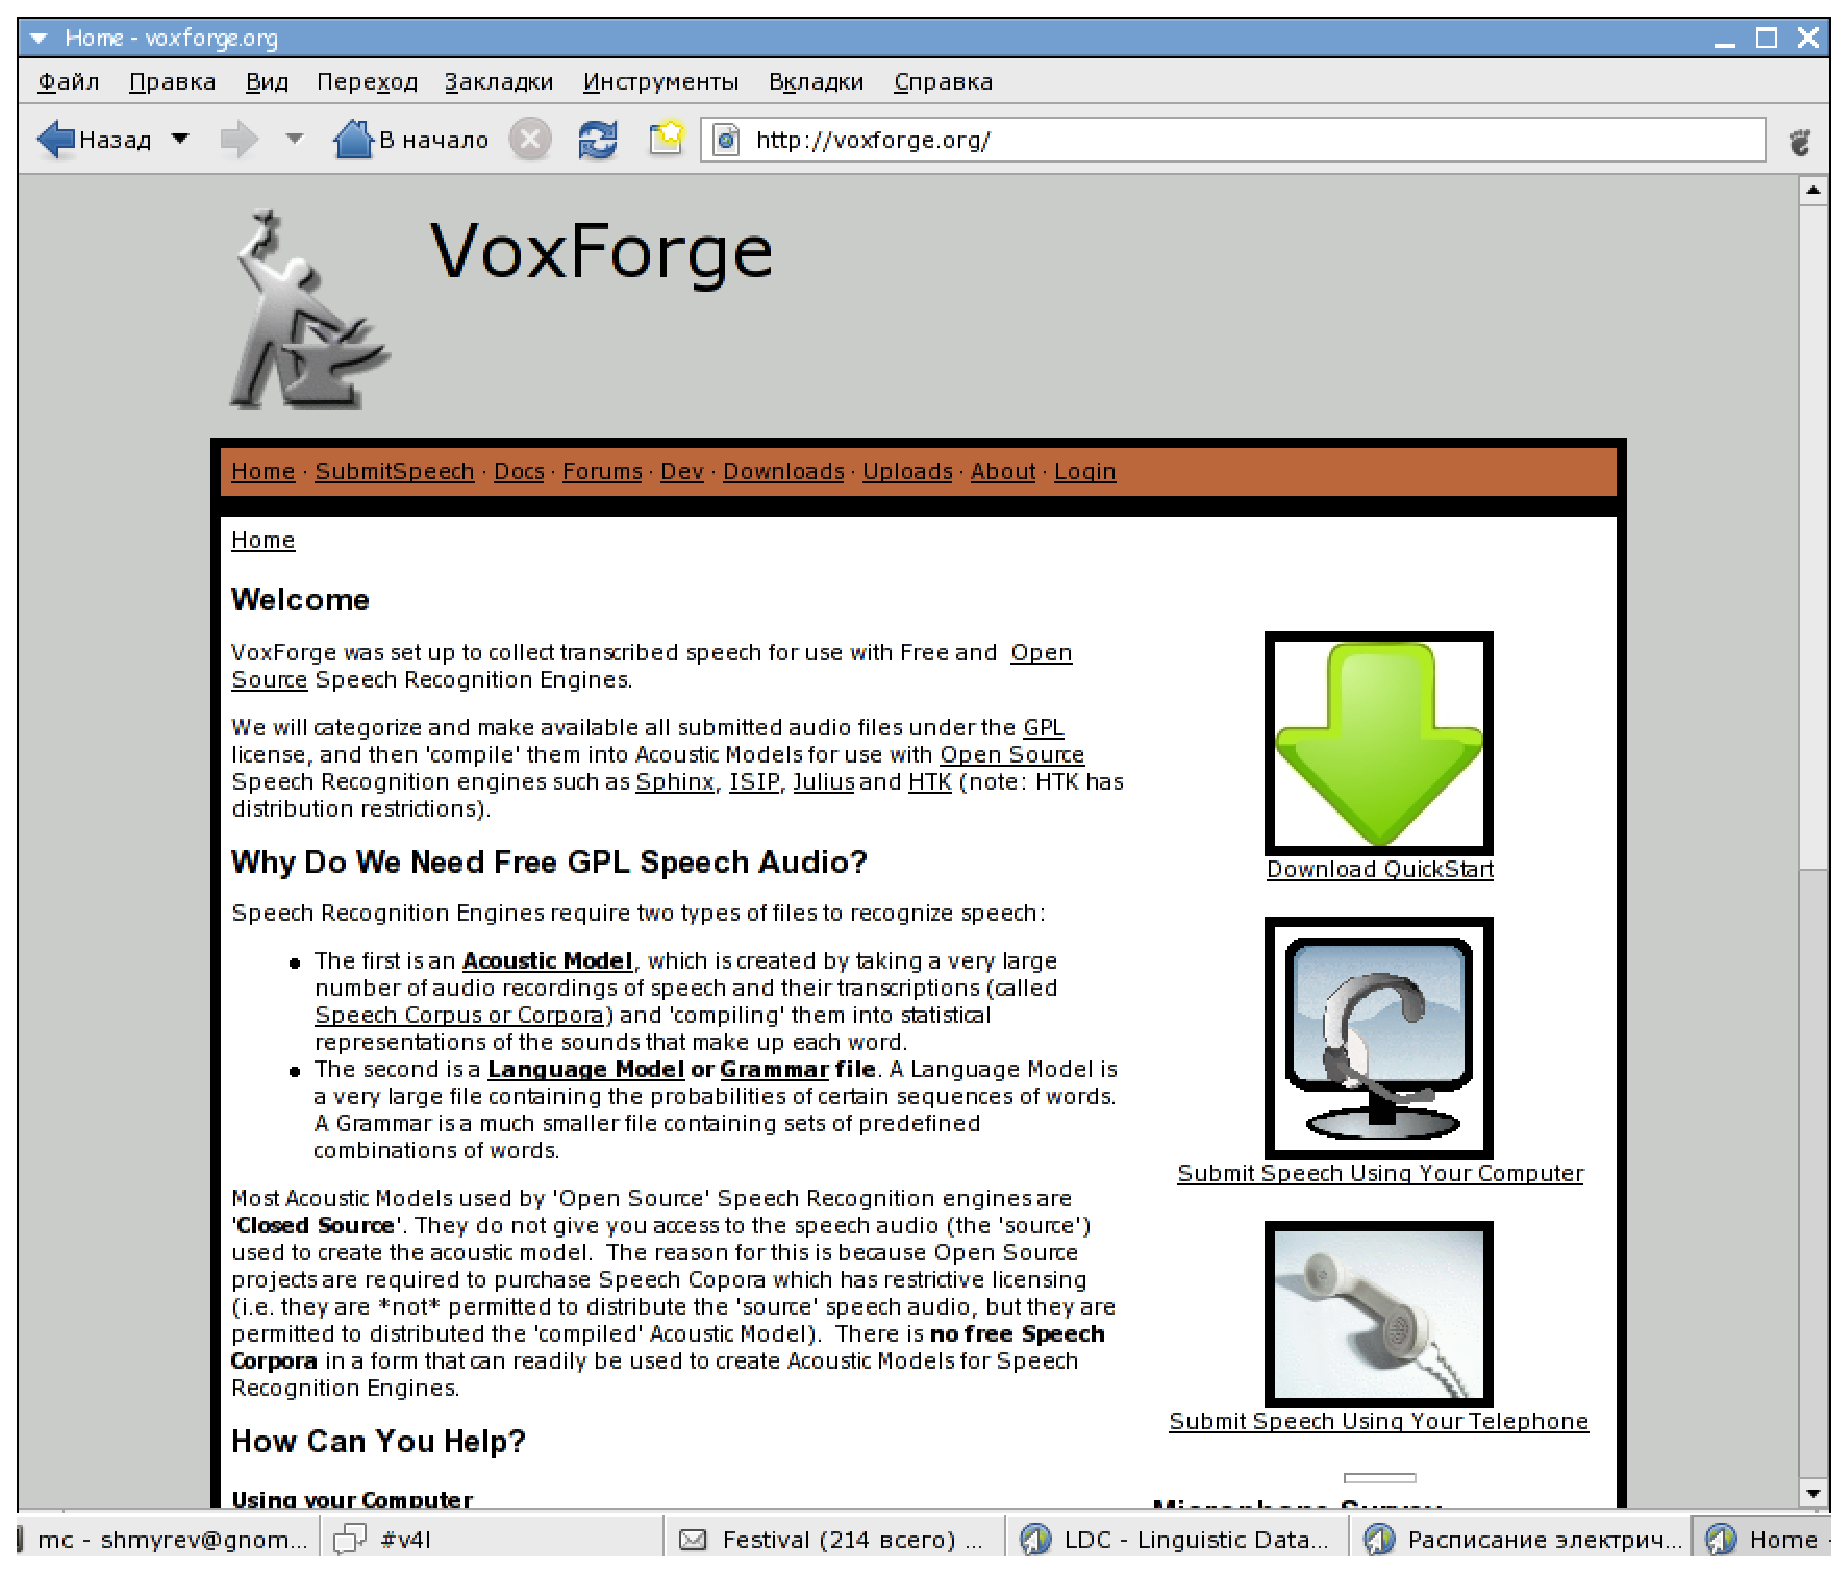
\includegraphics[width=.7\textwidth]{./images/voxforge.eps}
\end{center}
\end{figure}

\end{slide}


\begin{slide}
gnome-voice-control. Проект в рамках Google SOC

\begin{itemize}
\item Управление рабочим столом
\item Управление приложениями
\item Диктовка
\item Поддержка нескольких языков
\end{itemize}

\end{slide}

\begin{slide}
Русский язык
 
Мужской и женский голоса для festival http://festlang.berlios.de/russian.html

База для распознавания - 10 дикторов (нужно 200). Точность распознавания
на тестовых данных -- 80\% точность слов, 50\% точность предложений.

http://www.dev.voxforge.org/projects/Russian

\end{slide}

\end{document}
